%%%%%%%%%%%%%%%%%%%%%%%%%%%%%%%%%%%%%%%%%%%%%%%%%
% Chapter: Query
%%%%%%%%%%%%%%%%%%%%%%%%%%%%%%%%%%%%%%%%%%%%%%%%%
\chapter{Query Operations}
\label{chap:api_proc_mgmt:query}

This chapter presents mechanisms for generalized queries that
access information about the host environment and the system in general.
The chapter presents the concept of a query followed by a detailed explanation 
of the queries \acp{API} provided.  The chapter compares the use of these \acp{API} with \refapi{PMIx_Get}.  The chapter concludes with detailed information about how to use
the query interface to access information about what \ac{PMIx} \acp{API} an implementation supports as well as what attributes each supported \ac{API} supports.

\section{PMIx_Query_info}
As the level of interaction between applications and the host \ac{SMS} grows, so too does the need for the application to query the \ac{SMS} regarding its capabilities and state information. \ac{PMIx} provides a generalized query interface for this purpose, along with a set of standardized attribute keys to support a range of requests. This includes requests to determine the status of scheduling queues and active allocations, the scope of \ac{API} and attribute support offered by the \ac{SMS}, namespaces of active jobs, location and information about a job's processes, and information regarding available resources.

An example use-case for the \refapi{PMIx_Query_info_nb} \ac{API} is to ensure clean job completion. Time-shared systems frequently impose maximum run times when assigning jobs to resource allocations. To shut down gracefully (e.g., to write a checkpoint before termination) it is necessary for an application to periodically query the resource manager for the time remaining in its allocation. This is especially true on systems for which allocation times may be shortened or lengthened from the original time limit. Many resource managers provide \acp{API} to dynamically obtain this information, but each \ac{API} is specific to the resource manager.  
\ac{PMIx} supports this use-case by defining an attribute key (\refattr{PMIX_TIME_REMAINING}) that can be used with the \refapi{PMIx_Query_info_nb} interface to obtain the number of seconds remaining in the current job allocation. 

\ac{PMIx} sometimes provides multiple methods by which an application can obtain information or services.  For this example, 
note that one could alternatively use the \refapi{PMIx_Register_event_handler} \ac{API} to register for an event indicating incipient job termination, and then use the \refapi{PMIx_Job_control_nb} \ac{API} to request that the host \ac{SMS} generate an event a specified amount of time prior to reaching the maximum run time. 

%%%%%%%%%%%%%%%%%%%%%%%%%%%%%%%%%%%%%%%%%%%%%%%%%
\subsection{Query Structure}
\declarestruct{pmix_query_t}

A \ac{PMIx} query structure is composed of one or more keys and a list of qualifiers which provide additional information to describe the query.
Keys which use the same qualifiers can be placed in the same query for compactness, though it is permissable to put each key in its own query.

The \refstruct{pmix_query_t} structure is used by the \refapi{PMIx_Query_info} \acp{API} to describe a single query operation.

\copySignature{pmix_query_t}{2.0}{
typedef struct pmix_query \{ \\
\hspace*{4\sigspace}char **keys; \\
\hspace*{4\sigspace}pmix_info_t *qualifiers; \\
\hspace*{4\sigspace}size_t nqual; \\
\} pmix_query_t;
}

where:

\begin{itemize}
    \item \emph{keys} is a \code{NULL}-terminated argv-style array of strings
    \item \emph{qualifiers} is an array of \refstruct{pmix_info_t} describing constraints on the query
    \item \emph{nqual} is the number of elements in the \refarg{qualifiers} array
\end{itemize}

The following \acp{API} support query of various session and environment values.

%%%%%%%%%%%%%%%%%%%%%%%%%%%%%%%%%%%%%%%%%%%%%%%%%
\subsection{\code{PMIx_Query_info}}
\declareapi{PMIx_Query_info}

%%%%
\summary

Query information about the system in general.

%%%%
\format

\copySignature{PMIx_Query_info}{4.0}{
pmix_status_t \\
PMIx_Query_info(pmix_query_t queries[], size_t nqueries, \\
\hspace*{16\sigspace}pmix_info_t *info[], size_t *ninfo);
}

\begin{arglist}
\argin{queries}{Array of query structures (array of handles)}
\argin{nqueries}{Number of elements in the \refarg{queries} array (integer)}
\arginout{info}{Address where a pointer to an array of \refstruct{pmix_info_t} containing the results of the query can be returned (memory reference)}
\arginout{ninfo}{Address where the number of elements in \refarg{info} can be returned (handle)}
\end{arglist}

A successful return indicates that all data was found and has been returned.

\returnstart
\begin{itemize}
\item \refconst{PMIX_ERR_NOT_FOUND} None of the requested data was available.
\item \refconst{PMIX_ERR_PARTIAL_SUCCESS} Some of the requested data was found.
The \refarg{info} array shall contain an element for each query key that returned a value.
\end{itemize}
\returnend

If a value other than \refconst{PMIX_SUCCESS} or \refconst{PMIX_ERR_PARTIAL_SUCCESS} is returned, the
\refarg{info} array shall be \code{NULL} and \refarg{ninfo} zero.

\reqattrstart
A call to this \ac{API} can specify multiple queries.  Each query is composed of a list of keys and a list of attributes which can influence that query.  \ac{PMIx} libraries and host environments that support this \ac{API} are required to support the following attributes which are specified on a per-query basis:

\pasteAttributeItem{PMIX_QUERY_REFRESH_CACHE}
\pasteAttributeItem{PMIX_SESSION_INFO}
\pasteAttributeItem{PMIX_JOB_INFO}
\pasteAttributeItem{PMIX_APP_INFO}
\pasteAttributeItem{PMIX_NODE_INFO}
\pasteAttributeItem{PMIX_PROC_INFO}
\pasteAttributeItemBegin{PMIX_PROCID}In this context, specifies the process ID whose information is being requested - e.g., a query asking for the \refstruct{pmix_proc_info_t} of a specified process. Only required when the request is for information on a specific process.
\pasteAttributeItemEnd
\pasteAttributeItemBegin{PMIX_NSPACE}Specifies the namespace of the process whose information is being requested. Must be accompanied by the \refattr{PMIX_RANK} attribute. Only required when the request is for information on a specific process.
\pasteAttributeItemEnd
\pasteAttributeItemBegin{PMIX_RANK}Specifies the rank of the process whose information is being requested. Must be accompanied by the \refattr{PMIX_NSPACE} attribute. Only required when the request is for information on a specific process.
\pasteAttributeItemEnd
\pasteAttributeItem{PMIX_QUERY_ATTRIBUTE_SUPPORT}
\pasteAttributeItem{PMIX_CLIENT_ATTRIBUTES}
\pasteAttributeItem{PMIX_SERVER_ATTRIBUTES}
\pasteAttributeItem{PMIX_HOST_ATTRIBUTES}
\pasteAttributeItem{PMIX_TOOL_ATTRIBUTES}

Note that inclusion of both the \refattr{PMIX_PROCID} directive and either the \refattr{PMIX_NSPACE} or the \refattr{PMIX_RANK} attribute will return a \refconst{PMIX_ERR_BAD_PARAM} result, and that the inclusion of a process identifier must apply to all keys in that \refstruct{pmix_query_t}. Queries for information on multiple specific processes therefore requires submitting multiple \refstruct{pmix_query_t} structures, each referencing one process.  Directives which are not applicable to a key are ignored. 

% Use of pmix_server_query_fn is covered in server interfaces chapter
\reqattrend

An implementation is not required to support any keys.  If a key is unsupported, the implementation should handle that key in the same way that it is required to handle a key which it cannot find.
The following keys may be specified in a query:

\pasteAttributeItem{PMIX_QUERY_ATTRIBUTE_SUPPORT}
\pasteAttributeItem{PMIX_QUERY_NAMESPACES}
\pasteAttributeItem{PMIX_QUERY_JOB_STATUS}
\pasteAttributeItem{PMIX_QUERY_QUEUE_LIST}
\pasteAttributeItem{PMIX_QUERY_QUEUE_STATUS}
\pasteAttributeItem{PMIX_QUERY_PROC_TABLE}
\pasteAttributeItem{PMIX_QUERY_LOCAL_PROC_TABLE}
\pasteAttributeItem{PMIX_QUERY_SPAWN_SUPPORT}
\pasteAttributeItem{PMIX_QUERY_DEBUG_SUPPORT}
\pasteAttributeItem{PMIX_QUERY_MEMORY_USAGE}
\pasteAttributeItem{PMIX_QUERY_REPORT_AVG}
\pasteAttributeItem{PMIX_QUERY_REPORT_MINMAX}
\pasteAttributeItem{PMIX_QUERY_ALLOC_STATUS}
\pasteAttributeItem{PMIX_TIME_REMAINING}
\pasteAttributeItemBegin{PMIX_SERVER_URI} Requests the URI of the specified \ac{PMIx} server's \ac{PMIx} connection. Defaults to requesting the information for the local \ac{PMIx} server.
\pasteAttributeItemEnd
\pasteAttributeItem{PMIX_CLIENT_AVG_MEMORY}
\pasteAttributeItem{PMIX_DAEMON_MEMORY}
\pasteAttributeItem{PMIX_QUERY_AUTHORIZATIONS}
\pasteAttributeItem{PMIX_PROC_PID}
\pasteAttributeItem{PMIX_PROC_STATE_STATUS}

%%%%
\descr

Query information about the system in general.
This can include a list of active namespaces, fabric topology, etc.
Also can be used to query node-specific info such as the list of peers executing on a given node. The host environment is responsible for exercising appropriate access control on the information.

The returned \refarg{status} indicates if requested data was found or not. The returned \refarg{info} array will contain a \refattr{PMIX_QUERY_RESULTS} element for each query of the \refarg{queries} array. If qualifiers were included in the query, then the first element of each results array shall contain the \refattr{PMIX_QUERY_QUALIFIERS} key with a \refstruct{pmix_data_array_t} containing the qualifiers. The remaining \refstruct{pmix_info_t} shall contain the results of the query, one entry for each key that was found. Note that duplicate keys in the \refarg{queries} array shall result in duplicate responses within the constraints of the accompanying qualifiers. The caller is responsible for releasing the returned array.

\adviceimplstart
It is recommended that information returned from \refapi{PMIx_Query_info} be locally cached so that retrieval by subsequent calls to \refapi{PMIx_Get}, \refapi{PMIx_Query_info}, or \refapi{PMIx_Query_info_nb} can succeed with minimal overhead. The local cache shall be checked prior to querying the \ac{PMIx} server and/or the host environment. Queries that include the \refattr{PMIX_QUERY_REFRESH_CACHE} attribute shall bypass the local cache and retrieve a new value for the query, refreshing the values in the cache upon return.
\adviceimplend


%%%%%%%%%%%%%%%%%%%%%%%%%%%%%%%%%%%%%%%%%%%%%%%%%
\subsection{\code{PMIx_Query_info_nb}}
\declareapi{PMIx_Query_info_nb}

%%%%
\summary

Query information about the system in general.

%%%%
\format

\copySignature{PMIx_Query_info_nb}{2.0}{
pmix_status_t \\
PMIx_Query_info_nb(pmix_query_t queries[], size_t nqueries, \\
\hspace*{19\sigspace}pmix_info_cbfunc_t cbfunc, void *cbdata);
}

\begin{arglist}
\argin{queries}{Array of query structures (array of handles)}
\argin{nqueries}{Number of elements in the \refarg{queries} array (integer)}
\argin{cbfunc}{Callback function \refapi{pmix_info_cbfunc_t} (function reference)}
\argin{cbdata}{Data to be passed to the callback function (memory reference)}
\end{arglist}

A successful return indicates that the request has been accepted for processing.
The provided callback function will only be executed upon successful return of the operation.
Note that the library must not invoke the callback function prior to returning from the \ac{API}.

\returnsimple

If executed, the status returned in the provided callback function will be one of the following constants:

\begin{itemize}
\item \refconst{PMIX_SUCCESS} All data was found and has been returned.

\item \refconst{PMIX_ERR_NOT_FOUND} None of the requested data was available.
The \refarg{info} array will be \code{NULL} and \refarg{ninfo} zero.

\item \refconst{PMIX_ERR_PARTIAL_SUCCESS} Some of the requested data was found.
The \refarg{info} array shall contain an element for each query key that returned a value.

\item \refconst{PMIX_ERR_NOT_SUPPORTED} The host \ac{RM} does not support this function. The \refarg{info} array will be \code{NULL} and \refarg{ninfo} zero.

\item a non-zero \ac{PMIx} error constant indicating a reason for the request's failure. The \refarg{info} array will be \code{NULL} and \refarg{ninfo} zero.
\end{itemize}

\reqattrstart
\ac{PMIx} libraries and host environments that support this \ac{API} are required to support the following attributes:

\pasteAttributeItem{PMIX_QUERY_REFRESH_CACHE}
\pasteAttributeItem{PMIX_SESSION_INFO}
\pasteAttributeItem{PMIX_JOB_INFO}
\pasteAttributeItem{PMIX_APP_INFO}
\pasteAttributeItem{PMIX_NODE_INFO}
\pasteAttributeItem{PMIX_PROC_INFO}
\pasteAttributeItemBegin{PMIX_PROCID}In this context, specifies the process ID whose information is being requested - e.g., a query asking for the \refstruct{pmix_proc_info_t} of a specified process. Only required when the request is for information on a specific process.
\pasteAttributeItemEnd
\pasteAttributeItemBegin{PMIX_NSPACE}Specifies the namespace of the process whose information is being requested. Must be accompanied by the \refattr{PMIX_RANK} attribute. Only required when the request is for information on a specific process.
\pasteAttributeItemEnd
\pasteAttributeItemBegin{PMIX_RANK}Specifies the rank of the process whose information is being requested. Must be accompanied by the \refattr{PMIX_NSPACE} attribute. Only required when the request is for information on a specific process.
\pasteAttributeItemEnd
\pasteAttributeItem{PMIX_CLIENT_ATTRIBUTES}
\pasteAttributeItem{PMIX_SERVER_ATTRIBUTES}
\pasteAttributeItem{PMIX_HOST_ATTRIBUTES}
\pasteAttributeItem{PMIX_TOOL_ATTRIBUTES}

Note that inclusion of both the \refattr{PMIX_PROCID} directive and either the \refattr{PMIX_NSPACE} or the \refattr{PMIX_RANK} attribute will return a \refconst{PMIX_ERR_BAD_PARAM} result, and that the inclusion of a process identifier must apply to all keys in that \refstruct{pmix_query_t}. Queries for information on multiple specific processes therefore requires submitting multiple \refstruct{pmix_query_t} structures, each referencing one process.  Directives which are not applicable to a key are ignored. 

% Use of pmix_server_query_fn is covered in server interfaces chapter
\reqattrend

\optattrstart
An implementation is not required to support any keys.  If a key is unsupported, the implementation should handle that key in the same way that it is required to handle a key which it cannot find.
The following keys may be specified in a query:

\pasteAttributeItem{PMIX_QUERY_ATTRIBUTE_SUPPORT}
\pasteAttributeItem{PMIX_QUERY_NAMESPACES}
\pasteAttributeItem{PMIX_QUERY_JOB_STATUS}
\pasteAttributeItem{PMIX_QUERY_QUEUE_LIST}
\pasteAttributeItem{PMIX_QUERY_QUEUE_STATUS}
\pasteAttributeItem{PMIX_QUERY_PROC_TABLE}
\pasteAttributeItem{PMIX_QUERY_LOCAL_PROC_TABLE}
\pasteAttributeItem{PMIX_QUERY_SPAWN_SUPPORT}
\pasteAttributeItem{PMIX_QUERY_DEBUG_SUPPORT}
\pasteAttributeItem{PMIX_QUERY_MEMORY_USAGE}
\pasteAttributeItem{PMIX_QUERY_REPORT_AVG}
\pasteAttributeItem{PMIX_QUERY_REPORT_MINMAX}
\pasteAttributeItem{PMIX_QUERY_ALLOC_STATUS}
\pasteAttributeItem{PMIX_TIME_REMAINING}
\pasteAttributeItemBegin{PMIX_SERVER_URI} Requests the URI of the specified \ac{PMIx} server's \ac{PMIx} connection. Defaults to requesting the information for the local \ac{PMIx} server.
\pasteAttributeItemEnd
\pasteAttributeItem{PMIX_CLIENT_AVG_MEMORY}
\pasteAttributeItem{PMIX_DAEMON_MEMORY}
\pasteAttributeItem{PMIX_QUERY_AUTHORIZATIONS}
\pasteAttributeItem{PMIX_PROC_PID}
\pasteAttributeItem{PMIX_PROC_STATE_STATUS}

\optattrend

%%%%
\descr

Non-blocking form of the \refapi{PMIx_Query_info} \ac{API}.


%%%%%%%%%%%%%%%%%%%%%%%%%%%%%%%%%%%%%%%%%%%%%%%%%
%% NOTE: This is not used anywhere.  If this is supposed to be returned by
%% the query API's, it was never indicated.  They currently return 
%% PMIX_ERR_PARTIAL_SUCCESS
%%\subsection{Query-specific constants}
%%\label{api:struct:constants:query}

%%\begin{constantdesc}
%%%
%%\declareconstitemvalue{PMIX_QUERY_PARTIAL_SUCCESS}{-104}
%%Some, but not all, of the requested information was returned.
%%%
%%\end{constantdesc}


%%%%%%%%%%%%%%%%%%%%%%%%%%%%%%%%%%%%%%%%%%%%%%%%%
\subsection{Query keys}
\label{api:struct:key:query}

The following keys may be queried using the
\refapi{PMIx_Query_info} and \refapi{PMIx_Query_info_nb} \acp{API}:

%
\declareAttribute{PMIX_QUERY_SUPPORTED_KEYS}{"pmix.qry.keys"}{char*}{
Returns comma-delimited list of keys supported by the query function. NO QUALIFIERS.
}
%
\declareAttributeNEW{PMIX_QUERY_SUPPORTED_QUALIFIERS}{"pmix.qry.quals"}{char*}{
Return comma-delimited list of qualifiers supported by a query on the provided key, instead of actually performing the query on the key. NO QUALIFIERS.
}
%
\declareAttribute{PMIX_QUERY_NAMESPACES}{"pmix.qry.ns"}{char*}{
Request a comma-delimited list of active namespaces. NO QUALIFIERS.
}
%
\declareAttributeNEW{PMIX_QUERY_NAMESPACE_INFO}{"pmix.qry.nsinfo"}{pmix_data_array_t*}{
Return an array of active namespace information - each element will itself contain an array including the namespace plus the command line of the application executing within it. OPTIONAL QUALIFIERS: \refattr{PMIX_NSPACE} of specific namespace whose info is being requested.
}
%
\declareAttribute{PMIX_QUERY_JOB_STATUS}{"pmix.qry.jst"}{pmix_status_t}{
Status of a specified, currently executing job. REQUIRED QUALIFIER: \refattr{PMIX_NSPACE} indicating the namespace whose status is being queried.
}
%
\declareAttribute{PMIX_QUERY_QUEUE_LIST}{"pmix.qry.qlst"}{char*}{
Request a comma-delimited list of scheduler queues. NO QUALIFIERS.
}
%
\declareAttribute{PMIX_QUERY_QUEUE_STATUS}{"pmix.qry.qst"}{char*}{
Returns status of a specified scheduler queue, expressed as a string. OPTIONAL QUALIFIERS: \refattr{PMIX_ALLOC_QUEUE} naming specific queue whose status is being requested.
}
%
\pasteAttributeItem{PMIX_QUERY_PROC_TABLE}
%
\pasteAttributeItem{PMIX_QUERY_LOCAL_PROC_TABLE}
%
\declareAttribute{PMIX_QUERY_AUTHORIZATIONS}{"pmix.qry.auths"}{bool}{
Return operations the \ac{PMIx} tool is authorized to perform.  NO QUALIFIERS.
}
%
\declareAttribute{PMIX_QUERY_SPAWN_SUPPORT}{"pmix.qry.spawn"}{bool}{
Return a comma-delimited list of supported spawn attributes. NO QUALIFIERS.
}
%
\declareAttribute{PMIX_QUERY_DEBUG_SUPPORT}{"pmix.qry.debug"}{bool}{
Return a comma-delimited list of supported debug attributes. NO QUALIFIERS.
}
%
\declareAttribute{PMIX_QUERY_MEMORY_USAGE}{"pmix.qry.mem"}{bool}{
Return information on memory usage for the processes indicated in the qualifiers. OPTIONAL QUALIFIERS: \refattr{PMIX_NSPACE} and \refattr{PMIX_RANK}, or \refattr{PMIX_PROCID} of specific process(es) whose memory usage is being requested.
}
%
\declareAttribute{PMIX_TIME_REMAINING}{"pmix.time.remaining"}{char*}{
Query number of seconds (\code{uint32_t}) remaining in allocation for the specified namespace. OPTIONAL QUALIFIERS: \refattr{PMIX_NSPACE} of the namespace whose info is being requested (defaults to allocation containing the caller).
}
%
\declareAttributeNEW{PMIX_QUERY_ATTRIBUTE_SUPPORT}{"pmix.qry.attrs"}{bool}{
Query list of supported attributes for specified \acp{API}. REQUIRED QUALIFIERS: one or more of \refattr{PMIX_CLIENT_FUNCTIONS}, \refattr{PMIX_SERVER_FUNCTIONS}, \refattr{PMIX_TOOL_FUNCTIONS}, and \refattr{PMIX_HOST_FUNCTIONS}.
}
%
\pasteAttributeItem{PMIX_QUERY_NUM_PSETS}
%
\pasteAttributeItem{PMIX_QUERY_PSET_NAMES}
%
\pasteAttributeItem{PMIX_QUERY_PSET_MEMBERSHIP}
%
\declareAttributeNEW{PMIX_QUERY_AVAIL_SERVERS}{"pmix.qry.asrvrs"}{pmix_data_array_t*}{
Return an array of \refstruct{pmix_info_t}, each element itself containing a \refattr{PMIX_SERVER_INFO_ARRAY} entry holding all available data for a server on this node to which the caller might be able to connect.
}
%
\vspace{\baselineskip}
These keys are used to query memory available and used in the system.

%
\pasteAttributeItemBegin{PMIX_AVAIL_PHYS_MEMORY}OPTIONAL QUALIFERS: \refattr{PMIX_HOSTNAME} or \refattr{PMIX_NODEID} (defaults to caller's node).
\pasteAttributeItemEnd
%
\declareAttribute{PMIX_DAEMON_MEMORY}{"pmix.dmn.mem"}{float}{
Megabytes of memory currently used by the \ac{RM} daemon on the node. OPTIONAL QUALIFERS: \refattr{PMIX_HOSTNAME} or \refattr{PMIX_NODEID} (defaults to caller's node).
}
%
\declareAttribute{PMIX_CLIENT_AVG_MEMORY}{"pmix.cl.mem.avg"}{float}{
Average Megabytes of memory used by client processes on node. OPTIONAL QUALIFERS: \refattr{PMIX_HOSTNAME} or \refattr{PMIX_NODEID} (defaults to caller's node).
}

\vspace{\baselineskip}
The following attributes are used as qualifiers in queries regarding attribute support within the \ac{PMIx} implementation and/or the host environment:

\subsection{Query attributes}
\label{api:struct:attributes:query}

Attributes used to direct behavior of the 
\refapi{PMIx_Query_info} and \refapi{PMIx_Query_info_nb} \acp{API}:

\declareAttributeNEW{PMIX_QUERY_RESULTS}{"pmix.qry.res"}{pmix_data_array_t}{
Contains an array of query results for a given \refstruct{pmix_query_t} passed to the \refapi{PMIx_Query_info} \acp{API}. If qualifiers were included in the query, then the first element of the array shall be the \refattr{PMIX_QUERY_QUALIFIERS} attribute containing those qualifiers. Each of the remaining elements of the array is a \refstruct{pmix_info_t} containing the query key and the corresponding value returned by the query. This attribute is solely for reporting purposes and cannot be used in \refapi{PMIx_Get} or other query operations.
}
%
\declareAttributeNEW{PMIX_QUERY_QUALIFIERS}{"pmix.qry.quals"}{pmix_data_array_t}{
Contains an array of qualifiers that were included in the query that produced the provided results. This attribute is solely for reporting purposes and cannot be used in \refapi{PMIx_Get} or other query operations.
}
%
\declareAttribute{PMIX_QUERY_REFRESH_CACHE}{"pmix.qry.rfsh"}{bool}{
Retrieve updated information from server. NO QUALIFIERS.
}
%
\declareAttribute{PMIX_QUERY_LOCAL_ONLY}{"pmix.qry.local"}{bool}{
Constrain the query to local information only. NO QUALIFIERS.
}
%
\declareAttribute{PMIX_QUERY_REPORT_AVG}{"pmix.qry.avg"}{bool}{
Report only average values for sampled information. NO QUALIFIERS.
}
%
\declareAttribute{PMIX_QUERY_REPORT_MINMAX}{"pmix.qry.minmax"}{bool}{
Report minimum and maximum values. NO QUALIFIERS.
}
%
\declareAttribute{PMIX_QUERY_ALLOC_STATUS}{"pmix.query.alloc"}{char*}{
String identifier of the allocation whose status is being requested. NO QUALIFIERS.
}
%
\declareAttributeNEW{PMIX_SERVER_INFO_ARRAY}{"pmix.srv.arr"}{pmix_data_array_t}{
Array of \refstruct{pmix_info_t} about a given server, starting with its \refattr{PMIX_NSPACE} and including at least one of the rendezvous-required pieces of information.
}
%
\declareAttributeNEW{PMIX_CLIENT_FUNCTIONS}{"pmix.client.fns"}{bool}{
Request a list of functions supported by the \ac{PMIx} client library.
}
%
\declareAttributeNEW{PMIX_CLIENT_ATTRIBUTES}{"pmix.client.attrs"}{bool}{
Request attributes supported by the \ac{PMIx} client library.
}
%
\declareAttributeNEW{PMIX_SERVER_FUNCTIONS}{"pmix.srvr.fns"}{bool}{
Request a list of functions supported by the \ac{PMIx} server library.
}
%
\declareAttributeNEW{PMIX_SERVER_ATTRIBUTES}{"pmix.srvr.attrs"}{bool}{
Request attributes supported by the \ac{PMIx} server library.
}
%
\declareAttributeNEW{PMIX_HOST_FUNCTIONS}{"pmix.srvr.fns"}{bool}{
Request a list of functions supported by the host environment.
}
%
\declareAttributeNEW{PMIX_HOST_ATTRIBUTES}{"pmix.host.attrs"}{bool}{
Request attributes supported by the host environment.
}
%
\declareAttributeNEW{PMIX_TOOL_FUNCTIONS}{"pmix.tool.fns"}{bool}{
Request a list of functions supported by the \ac{PMIx} tool library.
}
%
\declareAttributeNEW{PMIX_TOOL_ATTRIBUTES}{"pmix.setup.env"}{bool}{
Request attributes supported by the \ac{PMIx} tool library functions.
}

%%%%%%%%%%%%%%%%%%%%%%%%%%%%%%%%%%%%%%%%%%%%%%%%%
\subsubsection{Query structure support macros}
The following macros are provided to support the \refstruct{pmix_query_t} structure.

%%%%
\littleheader{Static initializer for the query structure}
\declaremacroProvisional{PMIX_QUERY_STATIC_INIT}

Provide a static initializer for the \refstruct{pmix_query_t} fields.

\versionMarker{4.2}
\cspecificstart
\begin{codepar}
PMIX_QUERY_STATIC_INIT
\end{codepar}
\cspecificend

\littleheader{Initialize the query structure}
\declaremacro{PMIX_QUERY_CONSTRUCT}

Initialize the \refstruct{pmix_query_t} fields

\copySignature{PMIX_QUERY_CONSTRUCT}{2.0}{
PMIX_QUERY_CONSTRUCT(m)
}

\begin{arglist}
\argin{m}{Pointer to the structure to be initialized (pointer to \refstruct{pmix_query_t})}
\end{arglist}

\littleheader{Destruct the query structure}
\declaremacro{PMIX_QUERY_DESTRUCT}

Destruct the \refstruct{pmix_query_t} fields

\copySignature{PMIX_QUERY_DESTRUCT}{2.0}{
PMIX_QUERY_DESTRUCT(m)
}

\begin{arglist}
\argin{m}{Pointer to the structure to be destructed (pointer to \refstruct{pmix_query_t})}
\end{arglist}

%%%%%%%%%%%
\littleheader{Create a query array}
\declaremacro{PMIX_QUERY_CREATE}

Allocate and initialize an array of \refstruct{pmix_query_t} structures

\copySignature{PMIX_QUERY_CREATE}{2.0}{
PMIX_QUERY_CREATE(m, n)
}

\begin{arglist}
\arginout{m}{Address where the pointer to the array of \refstruct{pmix_query_t} structures shall be stored (handle)}
\argin{n}{Number of structures to be allocated (\code{size_t})}
\end{arglist}


%%%%%%%%%%%
\littleheader{Free a query structure}
\declaremacro{PMIX_QUERY_RELEASE}

Release a \refstruct{pmix_query_t} structure

\copySignature{PMIX_QUERY_RELEASE}{4.0}{
PMIX_QUERY_RELEASE(m)
}

\begin{arglist}
\argin{m}{Pointer to a \refstruct{pmix_query_t} structure (handle)}
\end{arglist}

%%%%%%%%%%%
\littleheader{Free a query array}
\declaremacro{PMIX_QUERY_FREE}

Release an array of \refstruct{pmix_query_t} structures

\copySignature{PMIX_QUERY_FREE}{2.0}{
PMIX_QUERY_FREE(m, n)
}

\begin{arglist}
\argin{m}{Pointer to the array of \refstruct{pmix_query_t} structures (handle)}
\argin{n}{Number of structures in the array (\code{size_t})}
\end{arglist}

%%%%%%%%%%%
\littleheader{Create the info array of query qualifiers}
\declaremacro{PMIX_QUERY_QUALIFIERS_CREATE}

Create an array of \refstruct{pmix_info_t} structures for passing query qualifiers, updating the \refarg{nqual} field of the \refstruct{pmix_query_t} structure.

\copySignature{PMIX_QUERY_QUALIFIERS_CREATE}{2.2}{
PMIX_QUERY_QUALIFIERS_CREATE(m, n)
}

\begin{arglist}
\argin{m}{Pointer to the \refstruct{pmix_query_t} structure (handle)}
\argin{n}{Number of qualifiers to be allocated (\code{size_t})}
\end{arglist}

%%%%%%%%%%%%%%%%%%%%%%%%%%%%%%%%%%%%%%%%%%%%%%%%%
\section{\code{PMIx_Resolve_peers}}

There are a number of common queries for which \ac{PMIx} provides convenience routines.
These \acp{API} provide similified access to commonly requested queries.  Due to their simplified interface, these \acp{API} cannot be customized through the use of attributes.
If a more specialized version of these queries are required, similar functionality can
often be accessed through the \refapi{PMIx_Query_info} or \refapi{PMIx_Query_info_nb} \acp{API}.

\declareapi{PMIx_Resolve_peers}

%%%%
\summary

Obtain the array of processes within the specified namespace that are executing on a given node.

%%%%
\format

\copySignature{PMIx_Resolve_peers}{1.0}{
pmix_status_t \\
PMIx_Resolve_peers(const char *nodename, \\
                   const pmix_nspace_t nspace, \\
                   pmix_proc_t **procs, size_t *nprocs);
}

\begin{arglist}
\argin{nodename}{Name of the node to query - \code{NULL} can be used to denote the current local node (string)}
\argin{nspace}{namespace (string)}
\argout{procs}{Array of process structures (array of handles)}
\argout{nprocs}{Number of elements in the \refarg{procs} array (integer)}
\end{arglist}

\returnsimple

%%%%
\descr

Given a \refarg{nodename}, return the array of processes within the specified \refarg{nspace}
that are executing on that node.
If the \refarg{nspace} is \code{NULL}, then all processes on the node will be returned.
If the specified node does not currently host any processes, then the returned array will be \code{NULL}, and \refarg{nprocs} will be zero.
The caller is responsible for releasing the \refarg{procs} array when done with it.
The \refmacro{PMIX_PROC_FREE} macro is provided for this purpose.


%%%%%%%%%%%%%%%%%%%%%%%%%%%%%%%%%%%%%%%%%%%%%%%%%
\subsection{\code{PMIx_Resolve_nodes}}
\declareapi{PMIx_Resolve_nodes}

%%%%
\summary

Return a list of nodes hosting processes within the given namespace.

%%%%
\format

\copySignature{PMIx_Resolve_nodes}{1.0}{
pmix_status_t \\
PMIx_Resolve_nodes(const char *nspace, char **nodelist);
}

\begin{arglist}
\argin{nspace}{Namespace (string)}
\argout{nodelist}{Comma-delimited list of nodenames (string)}
\end{arglist}

Returns \refconst{PMIX_SUCCESS} or a negative value corresponding to a PMIx error constant.

%%%%
\descr

Given a \refarg{nspace}, return the list of nodes hosting processes within that namespace.
The returned string will contain a comma-delimited list of nodenames.
The caller is responsible for releasing the string when done with it.



%%%%%%%%%%%%%%%%%%%%%%%%%%%%%%%%%%%%%%%%%%%%%%%%%
%%%%%%%%%%%%%%%%%%%%%%%%%%%%%%%%%%%%%%%%%%%%%%%%%
\section{Using Get vs Query}
\label{chap:api_job_mgmt:query}

Both \refapi{PMIx_Get} and \refapi{PMIx_Query_info} can be used to retrieve information about the system. In general, the \emph{get} operation should be used to retrieve:

\begin{itemize}
\item information provided by the host environment at time of job start. This includes information on the number of processes in the job, their location, and possibly their communication endpoints.
\item information posted by processes via the \refapi{PMIx_Put} function.
\end{itemize}

This information is largely considered to be \emph{static}, although this will not necessarily be true for environments supporting dynamic programming models or fault tolerance. Note that the \refapi{PMIx_Get} function only accesses information about execution environments - i.e., its scope is limited to values pertaining to a specific \refterm{session}, \refterm{job}, \refterm{application}, \refterm{process}, or \refterm{node}. It cannot be used to obtain information about areas such as the status of queues in the \ac{WLM}.

In contrast, the \emph{query} option should be used to access:

\begin{itemize}
\item system-level information (such as the available \ac{WLM} queues) that would generally not be included in job-level information provided at job start.
\item dynamic information such as application and queue status, and resource utilization statistics. Note that the \refattr{PMIX_QUERY_REFRESH_CACHE} attribute must be provided on each query to ensure current data is returned.
\item information created post job start, such as process tables.
\item information requiring more complex search criteria than supported by the simpler \refapi{PMIx_Get} \ac{API}.
\item queries focused on retrieving multi-attribute blocks of data with a single request, thus bypassing the single-key limitation of the \refapi{PMIx_Get} \ac{API}.
\end{itemize}

In theory, all information can be accessed via \refapi{PMIx_Query_info} as the local cache is typically the same datastore searched by \refapi{PMIx_Get}. However, in practice, the overhead associated with the \emph{query} operation may (depending upon implementation) be higher than the simpler \emph{get} operation due to the need to construct and process the more complex \refstruct{pmix_query_t} structure. Thus, requests for a single key value are likely to be accomplished faster with \refapi{PMIx_Get} versus the \emph{query} operation.


%%%%%%%%%%%%%%%%%%%%%%%%%%%%%%%%%%%%%%%%%%%%%%%%%
%%%%%%%%%%%%%%%%%%%%%%%%%%%%%%%%%%%%%%%%%%%%%%%%%
\section{Accessing attribute support information}
\label{chap:api_job_mgmt:queryattrs}

Information as to which attributes are supported by either the \ac{PMIx} implementation or its host environment can be obtained via the \refapi{PMIx_Query_info} \acp{API}. The \refattr{PMIX_QUERY_ATTRIBUTE_SUPPORT} attribute must be listed as the first entry in the \refarg{keys} field of the \refstruct{pmix_query_t} structure, followed by the name of the function whose attribute support is being requested - support for multiple functions can be requested simultaneously by simply adding the function names to the array of \refarg{keys}. Function names \emph{must} be given as user-level \ac{API} names - e.g., ``PMIx_Get'', ``PMIx_server_setup_application'', or ``PMIx_tool_attach_to_server''.

The desired levels of attribute support are provided as qualifiers. Multiple levels can be requested simultaneously by simply adding elements to the \refarg{qualifiers} array. Each qualifier should contain the desired level attribute with the boolean value set to indicate whether or not that level is to be included in the returned information. Failure to provide any levels is equivalent to a request for all levels. Supported levels include:

\begin{itemize}
    \item \pasteAttributeItem{PMIX_CLIENT_FUNCTIONS}
    \item \pasteAttributeItem{PMIX_CLIENT_ATTRIBUTES}
    \item \pasteAttributeItem{PMIX_SERVER_FUNCTIONS}
    \item \pasteAttributeItem{PMIX_SERVER_ATTRIBUTES}
    \item \pasteAttributeItem{PMIX_HOST_FUNCTIONS}
    \item \pasteAttributeItem{PMIX_HOST_ATTRIBUTES}
    \item \pasteAttributeItem{PMIX_TOOL_FUNCTIONS}
    \item \pasteAttributeItem{PMIX_TOOL_ATTRIBUTES}
\end{itemize}

Unlike other queries, queries for attribute support can result in the number of returned \refstruct{pmix_info_t} structures being different from the number of queries. Each element in the returned array will correspond to a pair of specified attribute level and function in the query, where the \refarg{key} is the function and the \refarg{value} contains a \refstruct{pmix_data_array_t} of \refstruct{pmix_info_t}. Each element of the array is marked by a \refarg{key} indicating the requested attribute \emph{level} with a \refarg{value} composed of a \refstruct{pmix_data_array_t} of \refstruct{pmix_regattr_t}, each describing a supported attribute for that function, as illustrated in Fig. \ref{fig:attrquery} below where the requestor asked for supported attributes of \refapi{PMIx_Get} at the \refarg{client} and \refarg{server} levels, plus attributes of \refapi{PMIx_Allocation_request} at all levels.

\begingroup
\begin{figure*}[ht!]
  \begin{center}
    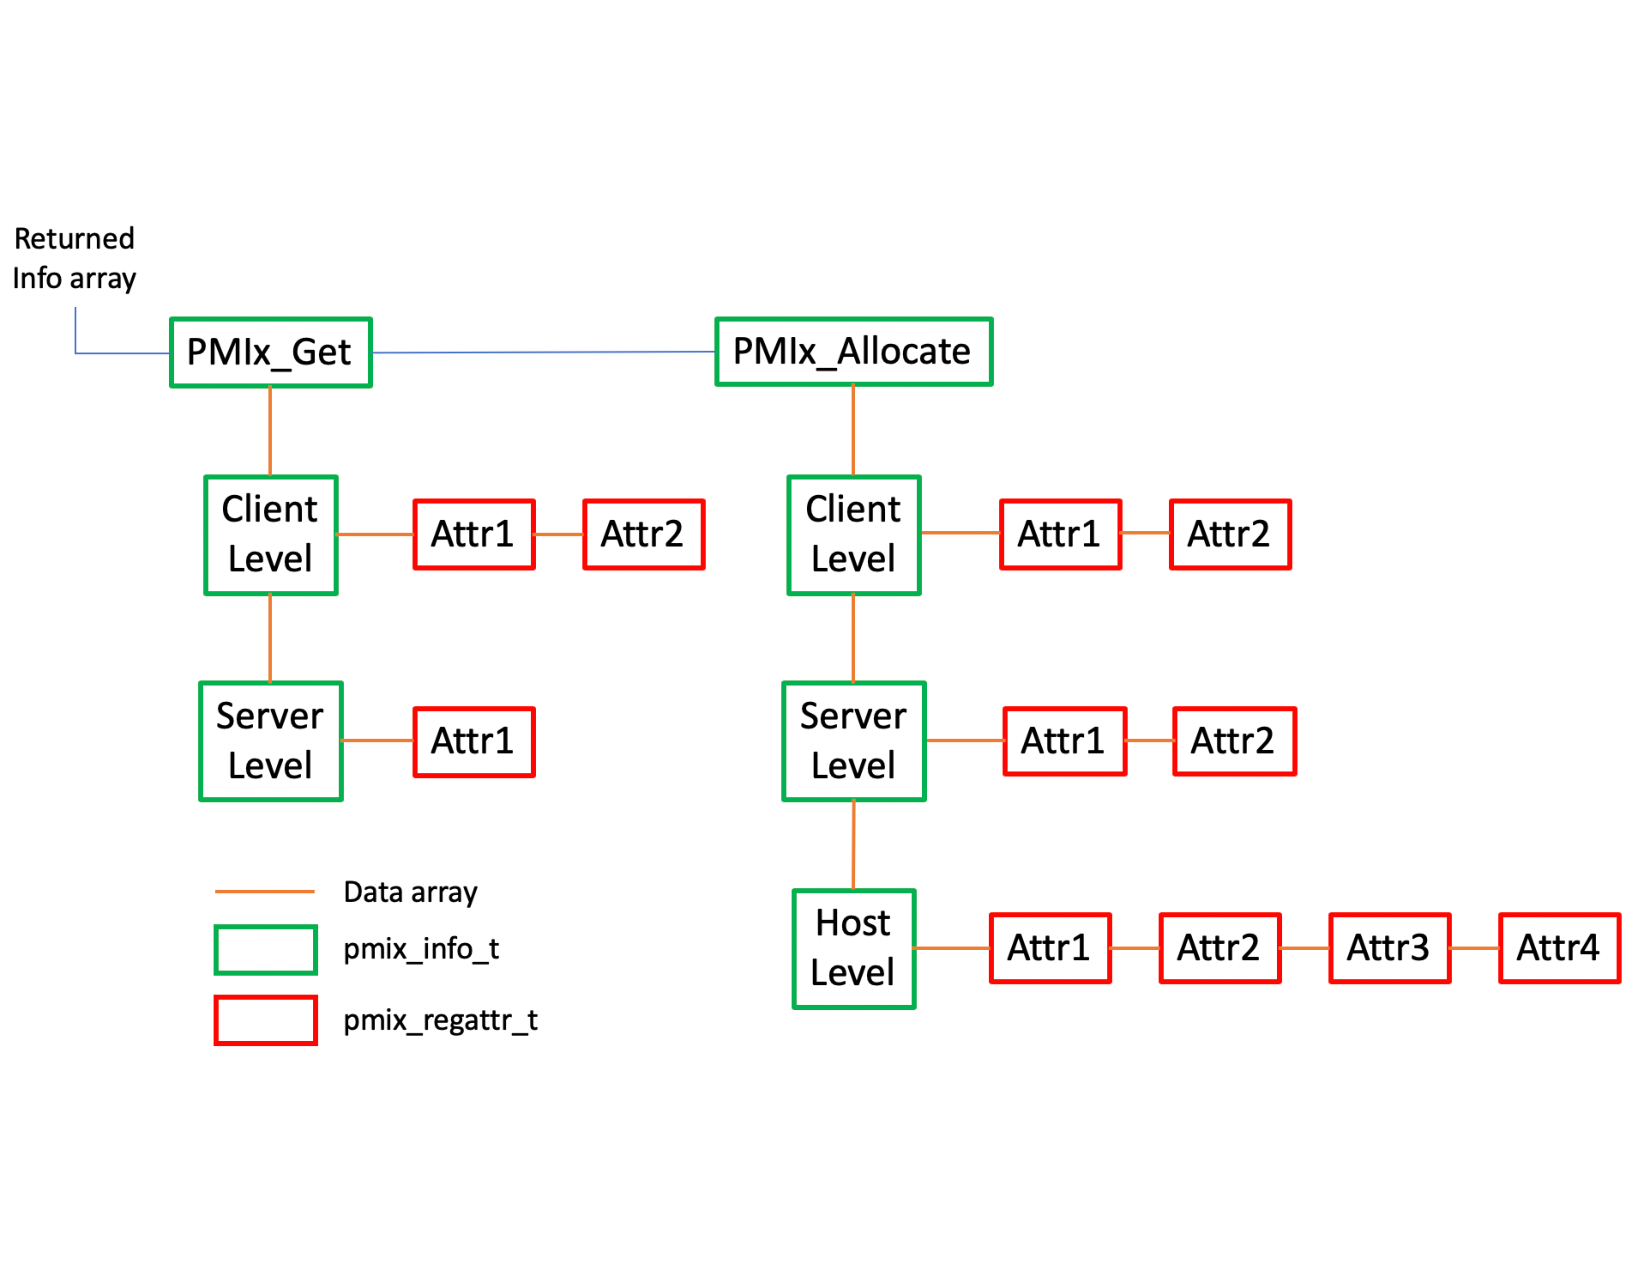
\includegraphics[clip,width=0.8\textwidth]{figs/attrquery.pdf}
  \end{center}
  \caption{Returned information hierarchy for attribute support request}
  \label{fig:attrquery}
\end{figure*}
\endgroup

The array of returned structures, and their child arrays, are subject to the return rules for the \refapi{PMIx_Query_info_nb} \ac{API}. For example, a request for supported attributes of the \refapi{PMIx_Get} function that includes the \refarg{host} level will return values for the \refarg{client} and \refarg{server} levels, plus an array element with a \refarg{key} of \refattr{PMIX_HOST_ATTRIBUTES} and a value type of \refconst{PMIX_UNDEF} indicating that no attributes are supported at that level.

%%%%%%%%%%%%%%%%%%%%%%%%%%%%%%%%%%%%%%%%%%%%%%%%%
